\documentclass{article}

\PassOptionsToPackage{numbers, compress}{natbib}

\usepackage[main,final]{neurips_2026}

\usepackage[utf8]{inputenc}
\usepackage[T1]{fontenc}
\usepackage[hidelinks]{hyperref}
\usepackage{url}
\usepackage{booktabs}
\usepackage{amsfonts}
\usepackage{amsmath}
\usepackage{graphicx}
\usepackage{nicefrac}
\usepackage{microtype}
\usepackage{caption}
\usepackage{xcolor}
\usepackage{upquote}

\newcommand{\pending}[1]{\textcolor{red}{[pending: #1]}}
\newcommand{\e}[1]{\times10^{-#1}}
\newcommand{\cn}[1]{\texttt{#1}}

\setcounter{topnumber}{4}
\setcounter{bottomnumber}{2}
\setcounter{totalnumber}{5}
\renewcommand{\topfraction}{0.95}
\renewcommand{\bottomfraction}{0.5}
\renewcommand{\textfraction}{0.06}
\renewcommand{\floatpagefraction}{0.7}

\title{Stop Heating an Empty Building: Reward Anatomy and a Supervisory Layer\\ for the NeurIPS 2026 Smart Buildings Challenge}

\author{%
  Semyon Morev\\
  Institute of Computer Science\\
  NUST MISIS, Moscow, Russia\\
  \texttt{m2508348@edu.misis.ru}
}

\begin{document}

\maketitle

\begin{abstract}
The NeurIPS 2026 Smart Buildings Challenge asks for one HVAC controller that runs, without
retraining, in commercial buildings it has never seen. We show that three properties of the
challenge's reward decide what such a controller should do. Comfort is charged as a mean over
the occupants present, so being ready when people arrive matters most and an empty building
need not be heated. A mandatory share of outdoor air and a capped supply temperature make heat
cheaper to deliver into a colder building, in one burst. And every zone holds the same number
of people, while the heat it needs grows with its floor area. Starting from Wu's public
adaptive-physics controller, we add a supervisory layer in three steps: a readiness ramp with a
release on days nobody comes; no heating of the empty building at night, above a frost floor;
and thirteen smaller mechanisms found by reading simulation traces, among them comfort margins
scaled by zone size. The result is $5.9\,\%$ better than the public controller on the simulator
with its billing errors corrected, and the thirteen mechanisms improve every one of 49 held-out
scenarios; on the public leaderboard the score moves from 0.01062 to 0.01002. We also measure
what missing information would be worth---a per-zone occupancy sensor about $3\,\%$, a perfect
weather forecast nothing---and audit the simulator's billing errors, which reward an exploit
and overcharge an honest controller by about $2\,\%$.
\end{abstract}

\section{Introduction}

The Smart Buildings Challenge \citep{goldfeder2026smart} evaluates controllers under a
protocol that makes transfer the whole problem: one policy is instantiated afresh for each
of 30 scenarios---six buildings crossed with five weather stations---and must run a month of
five-minute steps without retraining, network access or a site visit. Buildings have 30 to 85
zones and 3 to 9 air handlers, so even the size of the action changes from one scenario to the
next, and no physics, plant sizes or per-zone occupancy are exposed. A submission gets one
9-hour session for all 30 scenarios \citep{smartbuildings2026rules}. End-to-end reinforcement
learning is therefore expensive (about 107 CPU-hours for $5\times10^6$ PPO steps), and the
organizers report only single-digit-percent gains from SAC on one building
\citep{goldfeder2024smart}. Meanwhile the leaderboard is public, so the thing to beat is a
documented notebook: the strongest we found \citep{wu2026alpha075} scores seven times lower
(better) than the organizers' \cn{pid\_water} baseline. We port it exactly and ask what is
left to fix once a strong public controller is in hand.

\paragraph{What the reward implies.} The comfort penalty is averaged over the people present,
so the first person to arrive counts as much as a full building, and an empty building costs
nothing in comfort however cold it gets. The energy bill is the heat that reaches the zones
times a factor set by the minimum outdoor-air share and the cap on supply temperature
(Eq.~\ref{eq:mult}); the factor is smallest when the building is cold, so heat recovered in one
morning burst is cheaper than heat held all night. Together these say: do not heat an empty
building, and be ready when people arrive. The public controller we start from heats the empty
building all night, because its standby floor, held by the coldest zone of each air-handler
group, keeps the group's plant running until morning. CtrlW adds a readiness ramp and a release
for days nobody comes; CtrlW5 lowers that floor and cools the hot-water loop, which recovers
12.8 of the 93.1 units lost on the seven-day \emph{anchor} (\S\ref{sec:setting}), or 6.4 with
the frost floor we ship. A receding-horizon planner we built did not find this gain, so we
present it as a result about supervisory sequencing rather than control quality. CtrlX adds
thirteen smaller mechanisms found by reading simulation traces, worth another $2.9\,\%$, where
two evolutionary searches over the same knobs found nothing. The last of them comes from a third
property: every zone holds the same number of people, so a kelvin of comfort is worth the same
in a small zone and a large one, while the heat to buy it grows with floor area.

\paragraph{Contributions.} (1)~A reward anatomy: comfort is a per-occupant mean, and the bill
is envelope heat times a closed-form ventilation multiplier (\S\ref{sec:anatomy}). (2)~A
supervisory layer on the public controller in three steps (CtrlW, CtrlW5, CtrlX), with
ablations, a frost-floor cost curve and the refutations that bound it (\S\ref{sec:method}).
(3)~An evaluation on the 30 training scenarios, 49 held-out ones, both simulator versions,
reseeded occupancy and the leaderboard (\S\ref{sec:results}). (4)~A measured value of the
missing information and an audit of the simulator's billing in both directions
(\S\ref{sec:voi}, \S\ref{sec:integrity}). Code, per-scenario results and the study reports are
public.\footnote{\url{https://github.com/MorS1337/sb26-stop-heating}}

\section{The benchmark and related work}
\label{sec:setting}

A scenario is a partially observed Markov decision process over a temperature field, plant
parameters and hidden per-zone occupancy; the policy acts in
$\mathcal{A}=\mathbb{R}^{3H+2+2V}\times\{0,1\}^{H+1}$ (per handler a supply-air
temperature, a static-pressure setpoint and a recirculation fraction $r_k\le0.7$; two plant
values; per zone a damper floored at 10\,\% and a reheat valve), observes $6V+15H+58$ values
with zone readings lagged one step and \emph{one} building-level occupant count, but no
per-zone occupancy and no weather forecast; the plant cools centrally and heats only through
per-zone reheat coils. With live setpoints $T^{\text{lo}}_v,T^{\text{hi}}_v$ and
per-zone shortfall $s_{v,t}$ (linear to $w=5$\,K, quadratic beyond), the step reward and
score are $r_t=-0.6\,C_t-0.2\,\hat E_t-0.2\,\hat C_t\le0$ and
$S=\frac{1}{30}\sum_{s=1}^{30}\big|\tfrac1T\sum_{t=1}^{T}r_{s,t}\big|$, with $C_t$ the
occupancy-weighted shortfall of Eq.~\eqref{eq:mean} and $\hat E_t,\hat C_t$ metered
electricity-plus-gas cost and carbon normalized by the draw at rated power times $H$; lower
$S$ is better. One runaway zone therefore dominates an episode, and the denominators scale
with $H$, so one parameter set behaves consistently across building sizes.

\paragraph{Terms used throughout.} \cn{dev30} is the 30 training scenarios at full 30-day
length; the \emph{holdouts} are 49 scenarios on unseen generated buildings and unseen climates
(\S\ref{sec:results}). The \emph{anchor} is the seven-day \cn{fairbanks\_1} episode on which the
public forum compares controllers, reported as a total reward in \emph{units}
(Appendix~\ref{app:anchor}). The \emph{shipped} simulator is the starter kit as released; the
\emph{corrected} one adds two open pull requests that fix how it bills boiler gas (B1) and mixes
return air (B2), the two accounting \emph{seams} audited in \S\ref{sec:integrity}.

The challenge \citep{goldfeder2026smart} asks whether domain-specific models or generic
foundation models adapt better to unseen buildings, on the substrate of the Smart Buildings
Control Suite \citep{goldfeder2024smart} with its lightweight finite-difference simulator
\citep{goldfeder2023lightweight}; its authors concluded that aggregating a policy into a
static schedule retains most of its value \citep{goldfeder2024policyextraction} and that
better simple heuristics remain to be found \citep{goldfeder2025iccvw}, which is the line our result continues. Because the
leaderboard is public we measure against three notebooks rather than re-derive them---a
per-zone PI rule \citep{malyshev2026ztbest}, a residual PPO policy on it
\citep{alex2026residualppo}, and the analytic one-step search we adopt
\citep{wu2026alpha075}---all rule-based or one step deep. Transfer is formalized by Building2Building
\citep{taboga2026building2building} and attacked by GenTL \citep{raisch2025gentl} and BUILDA
\citep{krug2025builda}; in practice MPC is limited by the modelling it requires
\citep{drgona2020mpc}, so we keep the base controller's fixed per-zone model, online residual and
one-step search, which stands in for the reset sequences of Guideline 36 \citep{ashrae2024g36} and
trim-and-respond \citep{taylor2015trimrespond}.
Evolution strategies suit a slow deterministic simulator
\citep{hansen2016cmaes,salimans2017es}; CityLearn 2022 \citep{nweye2023citylearn} is the closest
precedent, and benchmark hygiene follows \citep{blum2021boptest,nagy2023tenquestions}.

% ---------------------------------------------------------------------------
% Section draft: the reward's structure (comfort mean + ventilation-bound bill).
% Standalone: guarded macros, so it compiles inside paper/main.tex and inside
% paper/sections_preview.tex.
% ---------------------------------------------------------------------------
\providecommand{\pending}[1]{\textcolor{red}{[pending: #1]}}
\providecommand{\e}[1]{\times10^{-#1}}

\section{Reward anatomy}
\label{sec:anatomy}

\paragraph{Comfort is a mean over the people present.} For zone $v$
with live band $[T^{\text{lo}}_v,T^{\text{hi}}_v]$ and shortfall $s_{v,t}$ (linear to
$5$\,K, quadratic beyond), the productivity term of the reward is
\begin{equation}
\frac{P-P^{\min}}{P^{\max}-P^{\min}}-1
\;=\;-\,\frac{\sum_v o_{v,t}\,s_{v,t}}{\sum_v o_{v,t}},
\label{eq:mean}
\end{equation}
the occupancy-weighted \emph{mean} shortfall over the occupants present
\citep{goldfeder2026smart}. Because it is a mean, the headcount cancels: a kelvin of shortfall
costs the same with two people in the building as with sixty, so the first arrivals of the
morning cost as much as a full building, and an empty building costs nothing. Occupancy is
exogenous: every zone holds the same headcount, people arrive between 06:00 and 12:00 and leave
between 13:00 and 19:00, and a controller that only reacts to arrivals pays at every morning
mode change. % src: docs/sim_analysis.md L192-198, L341-343
The base controller is more reactive than its parameters suggest: its preheat ramp sits inside a
flag that is true only in the hour before the mode change, so its ramps never exceeded one hour.
Moving the ramp outside the flag at a 2\,h horizon cuts comfort regret in the first occupied hour
fivefold and improves the score by $1.0\,\%$; releasing a building that is still empty at noon
adds $0.77\,\%$ more, independently. Longer horizons keep improving that hour but not the score:
readiness saturates once every zone is in band, while the gas keeps growing. % src: results/{refwu_dev30_shipped,ctrw_all,ctrw_d3,ctrw_d4}

\paragraph{The bill is envelope heat times a ventilation multiplier.} On the anchor
(\texttt{building\_train\_1/fairbanks\_1}, 2\,016 steps, mean outside $-26.3\,^\circ$C) the same
controller loses $93.12$ units, almost all of them to energy and carbon; comfort is $0.6\,\%$.
% src: results/houssem_anchor_ctrlw; docs/opt_gap.md §3
Instrumenting the trajectory splits the bill: about three quarters is reheat that replaces the
heat the envelope loses, just under a quarter is the outside-air share of that same reheat, and
fans, the boiler's standing loss and the pump make up the last few percent
(Appendix~\ref{app:energy}). % src: results/ef_shipped/building_train_1__fairbanks_1.npz (2016 steps)
The outside-air share is fixed by the action space: recirculation is capped at $r\le0.7$, so at
least $30\,\%$ of the supply air comes from outside, and the coil must lift it from
$T_{\text{mix}}=0.7\,T_{\text{ret}}+0.3\,T_{\text{out}}$ to the discharge cap
$T_{\text{dis}}=308.15$\,K, while the zone receives only the drop from $T_{\text{dis}}$ to
$T_{\text{zone}}$. With $T_{\text{ret}}\approx T_{\text{zone}}$ this gives
\begin{equation}
\frac{\text{gas billed}}{\text{net zone heat}}\;=\;
1+\frac{0.3\,\big(T_{\text{zone}}-T_{\text{out}}\big)}{T_{\text{dis}}-T_{\text{zone}}},
\label{eq:mult}
\end{equation}
so at the anchor's ambient the multiplier is $2.00$ for a zone held at $294$\,K and $1.18$ for one
at $270$\,K (Figure~\ref{fig:mult}a): \emph{heat delivered into a colder building is cheaper}. A
controller cannot change the $0.3$, but it can choose the temperature at which it delivers the
morning recovery. Beyond that, the air side leaves little to gain: over the episode CtrlW pays
only about $1\,\%$ more gas per delivered watt than a coil at its cap would.
% src: docs/control_gap.md §0.2, §2 (eff.py: gas/Q_net exact identity); docs/opt_gap.md §2-3

\paragraph{What the anatomy rules out.} The exchange rate between the two terms rules out
trading comfort in occupied hours for energy. On the anchor $624$ of the $2{,}016$ steps have
someone in the building, and a uniform $1$\,K shortfall in those steps costs
$0.6\times(1/5)\times624\approx75$ units, while lowering the whole building by one kelvin saves
about $0.57$\,MWh of gas, or $1.9$ units: a ratio of about $39{:}1$. What remains is the time
nobody is there. The night costs nothing in comfort, yet CtrlW, like the family it comes from,
heats it.
% src: docs/control_gap.md §3; docs/opt_gap.md §6; docs/energy_flow.md "By time bucket"


\section{Method: from a public controller to a night release}
\label{sec:method}

\subsection{The base controller}

We adopt the public controller of \citet{wu2026alpha075} and port it exactly: with all our
flags off, our port reproduces its dev30 score to the last digit. It gives each zone a
first-order model whose coefficients are set from the zone's geometry and never updated, plus
a residual that tracks the one-step error. For each air handler it evaluates candidate pairs of
supply-air temperature and recirculation against those models, which makes it a one-step-deep
MPC; a small MLP ensemble corrects drift, and predicted gas is weighted 0.30 against
electricity. The controller is strong but plans neither the morning nor the night. Its standby
policy holds each zone between 282 and 307\,K, and because a group's plant runs when
\emph{any} zone of the group calls for heat, one cold zone keeps the whole group's plant on all
night.

\subsection{CtrlW: readiness, weights, guards}
\label{sec:ctrlw}

\paragraph{Readiness ramp.} The base controller ramps its band from the eco toward the comfort
window over \cn{precondition\_hours}, but the ramp lives inside the code path
guarded by \cn{comfort\_mode\_soon}---a flag true only in the 60 minutes before
comfort-mode onset---so any horizon longer than 1\,h was clamped by construction. We
run the same ramp outside the flag: from $h$ before the mode change $t_s$, each zone's lower bound is
$T^{\text{lo}}_{\text{eco}}+p(t)\,(T^{\text{lo}}-T^{\text{lo}}_{\text{eco}})+\mu$ with $p(t)=1-(t_s-t)/h$ and $\mu$ the
comfort margin (the upper bound alike), each step's request capped by the base controller's
recovery clamp at $1/1.5$ of the remaining gap; the one-step search tracks this band, and $h=2$\,h
is the tuned horizon.

\paragraph{Weights and guards.} Per unit of gas the reward charges $0.2\,(p_g+\lambda\kappa_g)$
and per unit of electricity $0.2\,(p_e+\lambda\kappa_e)$ ($p$ price, $\kappa$ carbon intensity,
$\lambda$ the ratio of the cost to the carbon normalizer, up to a common scale), so the
consistent weight of gas relative to electricity is $(p_g+\lambda\kappa_g)/(p_e+\lambda\kappa_e)$,
between 0.44 and 0.51 on the shipped scenarios. The base controller's 0.30 under-weights gas by
almost $40\,\%$. Correcting it barely moves the score, because gas is spent on reheat during
warm-up and electricity on fans and chillers during the day; we adopt the derived weight because
it is the correct objective, and claim no gain for it. Of the two guards, the occupancy-aware
release fires when the building is still empty at noon, which happens on public holidays; on
its own it improves the score by $0.77\,\%$, and \S\ref{sec:ctrlx} moves it to the morning. The
holiday guard never fires, because the schedule's own holiday list is empty.

\paragraph{What tuning the class buys.} Two variants of CtrlW change little: a per-zone horizon
(\emph{CtrlW2}, $-0.16\,\%$) and a fixed 2\,K pre-dawn lift for zones on the standby floor
(\emph{CtrlW4}, $-0.34\,\%$, better on 8 scenarios and worse on 10).\footnote{The other numbers
are refuted variants: CtrlW3 holds the band's exact edge or a warmer night floor
(\S\ref{sec:results}), CtrlW6 adds cooling-season levers (Appendix~\ref{app:cooling}) and CtrlW7
replaces the frost floor with a latch (\S\ref{sec:ctrlx}).}
% src: results/q8/ctw2_v4_dev30_kg and results/ctw4_dev30_shipped vs results/q8/ctrw_dev30_shipped_kg (all Kaggle, same platform)

\subsection{CtrlW5: do not heat an empty building}
\label{sec:ctrlw5}

Nobody is in the building at night (arrivals fall between 06:00 and 12:00), so the comfort term
charges nothing there. CtrlW nevertheless keeps the coldest zone of each air-handler group at
282\,K from 19:00 to 04:00, and with it the group's whole plant. CtrlW5 changes two numbers: it
lowers that standby floor to 262\,K, low enough that on the anchor it never binds, and it lowers
the hot-water target from 345 to 336\,K. Restoring both reproduces CtrlW4 bit-exactly. The floor
accounts for almost all of the gain (12.1 of the 12.8 anchor units); the cooler loop adds the
rest.

The trace shows three effects (Table~\ref{tab:anchor}, Figure~\ref{fig:mult}). First, the night
heating stops, while the building's mean temperature hardly moves: what changes is the coldest
zones and the plant. Second, the morning recovery becomes one burst at the discharge cap, and by
Eq.~\eqref{eq:mult} heat delivered into a colder building is cheaper. Third, the heat stored in
the fabric in the cheapest early-morning hours carries the building through much of the day,
because drifting down through the comfort band costs nothing. Gas falls by $14\,\%$, and comfort
gives back $0.6$ of the $12.8$ units; Appendix~\ref{app:anchor} splits the gain by term.

Two searches agree that this is the best point of the CtrlW family, although neither rules out a
better mechanism outside it. A 150-evaluation CMA-ES over CtrlW4's 16 supervisory knobs ends on
the lower bound of the standby floor, and releasing that bound brings it within $0.01$ units of
CtrlW5. A sweep of the floor alone, run at the CMA-ES optimum's other knobs, improves
monotonically down to 262\,K, below which the floor no longer binds. Its comfort term stays at
$-1.35$ from 274\,K down (CtrlW5, which keeps CtrlW4's other knobs, ends at $-1.12$), so the
gain is not bought with comfort in occupied hours.
% src: docs/control_gap.md §0, §2, §4-4.1, §4.3

\begin{figure}[t]
\centering
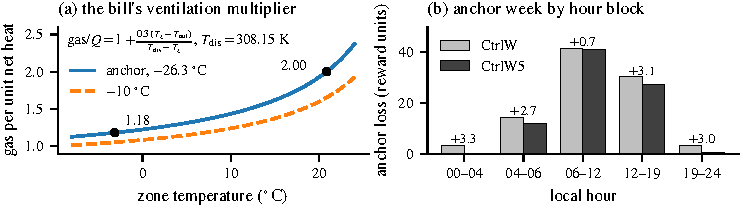
\includegraphics[width=0.76\linewidth]{figures/multiplier.pdf}
\caption{\textbf{(a)} The bill's ventilation multiplier, Eq.~\eqref{eq:mult}, at the
anchor's ambient ($-26.3\,^\circ$C) and at $-10\,^\circ$C: the same delivered heat costs
$2.00$ units of gas at a 294\,K zone and $1.18$ at 270\,K, which is why releasing the night
and recovering in one burst pays. \textbf{(b)} The anchor's loss by hour block: releasing the floor
removes $3.3$ (00--04), $2.7$ (04--06) and $3.0$ (19--24) units from the blocks the plant used to
heat, and $0.7$ and $3.1$ from the two daytime blocks, where the stored charge replaces coil duty.
Bar heights are losses (lower is better) and the labels are savings.}
\label{fig:mult}
% src: paper/figures/multiplier.py; hour blocks from docs/control_gap.md §2 (by_hour)
\end{figure}

\subsection{Frost protection, and what it costs}
\label{sec:frost}

Released completely, a building in Fairbanks freezes: on the anchor the coldest room falls to
$-8.6\,^\circ$C, and over a 30-day episode some room is below $0\,^\circ$C for 90 hours. The
simulator has no model of freezing and the score does not penalize it, so protecting the
building is our choice. We ship a \textbf{278\,K} floor ($4.85\,^\circ$C). It keeps every room
above $+4.5\,^\circ$C on the anchor and on the three cold 30-day scenarios, and the controller
still beats CtrlW by $6.9\,\%$ on the anchor and $3.8\,\%$ on the six Fairbanks scenarios
(Appendix~\ref{app:frost}). We measured this minimum on four scenarios; it is not guaranteed,
because the floor is a setpoint the controller can miss. Protection is expensive at the top of
the range and cheap at the bottom (Figure~\ref{fig:frost}): keeping every room at $5\,^\circ$C
or more needs a 280\,K floor and gives up 9.3 of the 12.8 units, while 274\,K already lets
rooms fall to $+0.6\,^\circ$C.
% src: docs/control_gap.md §8.1-8.3; paper/figures/frost.py
% src: results/frostburst_anchor/*.json (policies/ctrl_w7.py, 2016 steps, shipped, Mac)

\subsection{CtrlX: thirteen mechanisms read from traces}
\label{sec:ctrlx}

We then developed CtrlW5-278 further under a fixed protocol. Every candidate was scored on a
benchmark of ten seven-day scenarios on the corrected simulator with a non-default occupancy
seed; the module had to stay numpy-only, read no building or weather name, keep every room above
$+4\,^\circ$C and leave both accounting seams alone; and every change we kept was confirmed on
paired 30-day runs. Two CMA-ES searches over 14 of its knobs found nothing; every gain came
instead from reading simulation traces until they showed a mechanism. Table~\ref{tab:ctrlx}
(Appendix~\ref{app:ctrlx}) lists the thirteen mechanisms with a leave-one-out ablation; three of
them follow from \S\ref{sec:anatomy}.

\emph{(i) Holiday release.} The schedule runs comfort mode on every weekday, but the occupancy
model keeps people home on public holidays (in 23 of the 30 \cn{dev30} windows the building is
still empty at noon on some day), and the inherited release waits until noon. Arrivals come at
about $1/36$ per occupant per step, so a building still empty $K=\lceil330/V\rceil$ steps after
the mode change will stay empty that day, with a false-release probability below $10^{-4}$.
Releasing it then is the largest single mechanism ($1.0\,\%$).

\emph{(ii) A late start when the fabric is still warm.} The zone air heats and cools within a
step or two, while the fabric changes by less than a tenth of a kelvin per step. A ramp before
arrival therefore mostly charges the fabric at a low air temperature, which is cheap in deep cold
by Eq.~\eqref{eq:mult}, but every step of it also ventilates every zone of the group at the
minimum airflow. Both the benefit and the cost grow with the indoor--outdoor difference, so
whether the ramp pays depends only on how much heat the fabric still holds: to first order, it
stops paying once the group's mean temperature is within 2--5\,K of the setpoint
(Appendix~\ref{app:ctrlx}). CtrlX skips the 2--3\,h ramp for a group that is within 6\,K when the
window opens and keeps only the base controller's last hour. The same picture explains two
failures. Heating in bursts cannot replace the frost floor, because between bursts the air falls
back toward a fabric that sits below the floor (four designs and an earlier latch, CtrlW7, all
lose). And asking the one-step inversion for more than its clamped step, to arrive on time,
loses $0.4$--$53\,\%$.

\emph{(iii) Margins scaled by zone size.} Eq.~\eqref{eq:mean} weighs a zone by its occupants,
and every zone holds the same number, so a kelvin of shortfall costs the same in a 40\,m$^2$ zone
as in a 360\,m$^2$ one, while the heat that prevents it grows with floor area, which varies
3.5--9-fold within one building. CtrlX therefore scales each zone's comfort margin and arrival
lead, until then uniform, by $(\bar A/A_v)^{1/2}$, the square root of the median zone area over
the zone's own, clipped to $[\tfrac13,3]$. On the benchmark comfort, energy and carbon then
improve together, where every uniform change of margin or lead had traded one for the other;
exponents from 0.25 to 0.5 perform within $0.01\,\%$ of each other, and 1.0 overshoots.
% src: docs/ctrlx_experiments.md (mechanism table; runs #3, #49, #52; 2026-11-09/11 logs); zone areas as policies/ctrl_x.py derives them from the floor plan

\section{Results}
\label{sec:results}

\paragraph{Protocol.} \cn{dev30} (8{,}641 steps per scenario) is what the leaderboard draws
from; \cn{gen} is 32 scenarios from eight generated buildings under weather windows absent from
tuning; \cn{ext} replays those buildings and two shipped ones under 17 Meteostat 2023 stations
absent from the benchmark (Appendix~\ref{app:weather}). Scores are means over scenarios of
$|\tfrac1T\sum_t r_t|$, and comparisons against a base are paired. Reseeding occupancy moves a
score by at most $0.18\,\%$ and a paired gain by at most $0.12$ percentage points, so we read
only larger differences as gains. Numbers are for the shipped simulator unless marked
corrected. We report both, because the organizers aim to run final verification on the
corrected simulator \citep{rai2026verification,stncsn2026pr2,stncsn2026pr3} with a new occupancy
seed \citep{rai2026seed}, and we tune against neither the seams nor the seed. The CtrlX runs use
an exact C implementation of the simulator step, bit-identical in observations and rewards and
$1.6$--$2.1\times$ faster (Appendix~\ref{app:tools}).

\begin{table}[t]
\centering
\caption{Main comparison; score $S$ (lower is better). \cn{dev30} is 30 shipped scenarios at
8{,}641 steps, \cn{gen} 32 held-out generated scenarios and \cn{ext} 17 unseen climates (shipped tree);
\emph{shipped}/\emph{corrected} are the two simulator trees. CtrlX is the controller we ship; both it and
CtrlW5-278 keep a 278\,K night floor, CtrlW5-262 does not. The tank hold responds to the
shipped accounting and is reported apart (\S\ref{sec:integrity}). Public rows are the authors'
leaderboard scores unless we re-ran the controller.}
% src: results/{pid_water_dev30_shipped+pid_water_dev30_shipped_dstfix (25+5 scenarios),pidw_dev30_corrected,pidw_holdouts_shipped,refzt_dev30_shipped,refzt_dev30_corrected,refzt_holdouts_shipped+refzt_holdouts_shipped_fill (29+20=49 scenarios; gen 32 / ext 17 means computed per scenario),refwu_dev30_shipped,wu_dev30_corrected,refwu_gen_hold_shipped,refwu_ext_hold_shipped,ctrw_all,ctrw_all_corr,ctrw_holdouts_shipped,ctw4_dev30_shipped,ctw4_dev30_corrected,ctw4_holdouts_shipped,ctw5frost_dev30_shipped,ctw5frost_dev30_corrected,ctw5frost_holdouts_shipped,ctw5_dev30_shipped,ctw5_dev30_corrected,ctw5_holdouts_shipped}/summary.json
\label{tab:main}
\small
\setlength{\tabcolsep}{2pt}
\begin{tabular}{@{}lcccc@{}}
\toprule
Method & dev30 shipped & dev30 corrected & gen / ext & Kaggle public \\
\midrule
\cn{pid\_water} & 0.05498 & 0.05789 & 0.03620 / 0.05189 & --- \\
per-zone PI \citep{malyshev2026ztbest} & 0.01042 & 0.01023 & 0.007673 / 0.010748 & 0.01420 \\
Wu \citep{wu2026alpha075} & 0.0075040 & 0.0072641 & 0.005293 / 0.008015 & 0.01062 \\
CtrlW & 0.0073694 & 0.0071449 & 0.005179 / 0.007836 & 0.01051 \\
CtrlW4 & 0.0073445 & 0.0071587 & 0.005170 / 0.007813 & 0.01049 \\
CtrlW5-278 & 0.0071980 & 0.0070409 & 0.005058 / 0.007616 & 0.01032 \\
CtrlW5-262 (no frost floor) & 0.0071338 & 0.0069430 & 0.005052 / 0.007577 & 0.01024 \\
\textbf{CtrlX} & \textbf{0.0069712} & \textbf{0.0068387} & \textbf{0.004840 / 0.007353} & \textbf{0.01002} \\
\midrule
CtrlX $+$ tank hold & 0.0068269 & 0.0068420 & 0.004713 / 0.007173 & 0.00982 \\
\bottomrule
\end{tabular}
\end{table}

\paragraph{Main comparison.} Table~\ref{tab:main} gives every score. Each step of the
supervisory layer improves on the one before, and the corrected simulator keeps the order,
except that CtrlW4 falls just behind CtrlW. Correcting the billing lowers every score by
$1.8$--$3.2\,\%$, except the organizer baseline's and the tank hold's, which get worse. On the
49 held-out scenarios CtrlW5-278 beats CtrlW on 38 and ties on the other 11 (sign test
$p<10^{-11}$), so its gain is not specific to the training scenarios. The unseen climates score
about half again worse than the same buildings under familiar weather, so the transfer gap comes
from the climate. The leaderboard keeps the same order at 1.36--1.44 times the offline scores,
which we use only as a consistency check, and the frost floor costs about as much there as
offline ($0.8\,\%$ against $0.9\,\%$).

\paragraph{CtrlX.} On the corrected simulator, where it was developed, CtrlX improves on
CtrlW5-278 by $2.87\,\%$ on dev30 (better on 29 of 30 scenarios) and by $3.65\,\%$ on the 49
held-out scenarios, better on all 49, from about $1\,\%$ in the hot months to $12\,\%$ in spring
and autumn. The gain is therefore larger away from the development set than on it. The two
mechanisms added last are small ($0.03\,\%$ and $0.06\,\%$), below what one score resolves under
reseeding, but each gives the same gain on the held-out scenarios as on dev30, and the size
scaling also helps under all three occupancy seeds of the benchmark; we keep them because the
comparisons are paired and one-sided. With occupancy reseeded, the late start and the drift clip
still improve dev30 by about $0.4\,\%$, on 16 scenarios and with no losses. On the shipped
simulator CtrlX improves dev30 by $3.2\,\%$, the held-out scenarios by $3.9\,\%$ and the
leaderboard score by $2.9\,\%$, from 0.01032 to 0.01002.
% src: results/ctrlx/{arx_sz_both05,arx_op_op310,arx_abl_gap6}_dev30_corrected, results/ctrlx/arx_hc_{w5,v3,v5,x,v7}_gen_hold-ext_hold_corrected, results/ctrlx/arx_seed{12345,777}_{x,b}_dev30_corrected, results/ctrlx/arx_p7*; results/kaggle_submissions.csv; docs/ctrlx_experiments.md "Validation and leaderboard"

\paragraph{The anchor.} On the anchor, CtrlW is 11.2 units behind the best public controller
that respects the physics \citep{stncsn2026pr2} (Table~\ref{tab:anchor}). Perfect per-zone
foresight would recover only 2.6 of them and the accounting seams almost none, and our own
receding-horizon planner on a 79-node model of the building scores below CtrlW and never finds
the release, even with its defects fixed. Releasing the night closes the whole gap: the same
controller then scores $-80.31$, past the best public number, or $-86.68$ with the frost floor we
ship, and CtrlX reaches $-84.63$ with the same floor.
% src: results/{cg_ctrlw_anchor,cg_ctrlw4_anchor,optg_mpc2_anchor,cg_mpc2_night,cg_mpc2_float,cg_w5_final,foi_anchor_lead5}/summary.json; docs/control_gap.md §1, §5; results/ctrlx/integrity_anchor_weeks_v7 (CtrlX)

\paragraph{Ablations, reseeds, and what loses.} Table~\ref{tab:abl} (Appendix~\ref{app:abl})
adds one change at a time up to CtrlW5, including the horizon sweep of \S\ref{sec:anatomy}.
Reseeding occupancy moves each score by at most $0.18\,\%$, and CtrlW5-278's gain over CtrlW
stays between $2.2$ and $2.3\,\%$ under all three seeds. Several ideas lose: the two band levers
of CtrlW3, holding the schedule's own setpoint ($1.53$ anchor units) and a warmer 285\,K night
floor ($6.9$ units); the receding-horizon planner; and, for CtrlX, every uniform way of buying
back the first hour after arrival. That hour is $0.8\,\%$ of CtrlX's dev30 bill, most of its
comfort share, but a longer lead costs more gas than it saves in comfort, and even the best of
three leads per scenario, chosen with hindsight, is worth only $0.02\,\%$
(Appendix~\ref{app:ctrlx}).
% src: results/{ctrw_all,ctrw_dev30_seed12345,ctrw_dev30_seed777,ctw5frost_dev30_shipped,q7/ctw5frost_dev30_seed12345,q7/ctw5frost_dev30_seed777}; docs/opt_gap.md §6; docs/control_gap.md §4-5; results/ctrlx/arx_ld_{l075,l100}_dev30_corrected

% ---------------------------------------------------------------------------
% Section draft: value of information (main-text version). The ladder table is
% Table~\ref{tab:voi} in Appendix~\ref{app:voi}.
% ---------------------------------------------------------------------------
\providecommand{\pending}[1]{\textcolor{red}{[pending: #1]}}
\providecommand{\e}[1]{\times10^{-#1}}

\section{What information is worth}
\label{sec:voi}

The observation space exposes one occupant count for the whole building, no per-zone
occupancy and no weather forecast, while comfort is charged per zone. We hand the same
controller each missing channel in turn---a per-zone occupancy sensor, a perfect weather
forecast, the realised schedule, Table~\ref{tab:voi}---and never submit any of them, so the
deltas bound the value of sensing rather than propose an entry. An oracle is an instrument only if it is transparent, and these are: a policy that receives the
payload and drops it reproduces an ordinary run to the last digit on two full episodes, so the
channel perturbs neither the occupancy draw nor the clock, and the forecast is exact rather than
noisy (it equals the sensor reading $h$ hours later to $1.4\e{5}$\,K, the float32 quantisation of
the observation). % src: docs/voi_oracle.md §1 "Non-perturbation proof", "Forecast alignment"

\emph{Zonal occupancy pays $2.9\,\%$.} Dropping each zone to standby 15\,min after its own
occupants leave, rather than waiting for the whole building to empty as CtrlW's
occupancy release does, improves full dev30 from
0.0073694 to 0.0071585 and the corrected tree from 0.0071449 to 0.0069403 (both
$-2.86\,\%$); on the ten-scenario subset it is $-2.30\,\%$, better on 10 of 10, recovering
$23.9$ reward units of energy plus carbon for $0.16$ units of extra comfort regret. Raising the
release floor from 282 to 289\,K moves the subset score by $0.09\,\%$ and keeps 10/10, so the
result is about \emph{which} zones are empty, not how cold they get.
% src: results/{voi_occ_dev30_shipped,voi_occ_dev30_corrected,voi_occ_mild,voi_occ_dev10_pc}; docs/voi_oracle.md §3

\emph{A perfect forecast is worth nothing on top of a clock rule.} A fixed 2\,K pre-dawn lift,
gated only on the clock, the comfort-day predicate and the zone sitting on its standby floor,
scores 0.0073463 on dev30 ($-0.31\,\%$), and 0.0071582 against CtrlW's 0.0071449 on the
corrected tree---a wash there (the same lift shipped inside CtrlW4 scores 0.0073445, the
difference being the adaptive horizon underneath). Driving that lift and the preheat horizon
from a perfect 12\,h forecast scores 0.0073572: $0.15\,\%$ \emph{worse} than the constant lift
on dev30 and $0.01\,\%$ better on the subset, so the information is worth zero to within our
resolution and can have either sign. The mechanism is gated on the zone's own state and on a comfort day
coming, and the horizon response is flat-topped around 2\,h; on both cooling stations the forecast
variant is bit-identical to the no-information one.
% src: results/{nightlift_dev30_shipped,nightlift_dev30_corrected,voi_fcst_dev30_shipped,voi_fcst_dev10_pc}; docs/voi_oracle.md §3-4

\emph{The schedule is worth twice the sensor, and the difference is the lag.} Per-zone
foreknowledge of the episode's own occupancy, used to give each zone its own window with a
5\,h preheat lead, scores 0.0112001 on the subset ($-6.04\,\%$, 10/10) and $-90.52$ on the
anchor ($+2.60$ units, $+2.79\,\%$), with $+0.48$ to $+2.76\,\%$ at leads of 2--8\,h; the same information delivered
five minutes late and without a calendar loses $3.7$ percentage points. Relaxing the band by 1\,K in zones nobody has
entered yet is the asymmetric bet against it: $-0.44\,\%$ of score, but only 5 of 10 scenarios
and comfort regret multiplied from $5.33$ to $39.64$.
% src: results/{foi_foresight10,foi_anchor_lead5,voi_occ_morning}; docs/voi_oracle.md §3, §9.3-9.4


% ---------------------------------------------------------------------------
% Section draft: benchmark integrity (main-text version, compact; the audit table
% and the definitions are in Appendix~\ref{app:integrity}).
% ---------------------------------------------------------------------------
\providecommand{\pending}[1]{\textcolor{red}{[pending: #1]}}
\providecommand{\e}[1]{\times10^{-#1}}

\section{Benchmark integrity}
\label{sec:integrity}

The reward is computed from a simulator whose cost accounting is not closed under the
policy's action space. Two seams are public and both have a proposed fix: the hot-water
tank is billed from its setpoint rather than from its burner (B1, \citep{stncsn2026pr2}), and
the return air is mixed by floor area rather than by airflow (B2, \citep{stncsn2026pr3}).
Neither fix is merged and the leaderboard runs the unfixed tree, so what each seam is
worth is a measurement, taken by an instrument that leaves every per-step reward bit-identical
(Appendix~\ref{app:integrity}). % src: docs/integrity_audit.md §2.3-2.4
% src: the Kaggle forum digest (not released) B1/B2; docs/integrity_audit.md §2

\emph{B1 rewards an exploit.} A probe that applies the published setpoint recipe on top of CtrlW
delivers the same reheat while $11.1$\,MWh of gas stops being billed and comfort does not move:
the anchor improves by $36.9$ units, $3.3$ times the gap to the best public score there. It is
pure accounting: on the corrected simulator the same probe is slightly \emph{worse}. Over dev30,
gated to the heating periods, the recipe lowers CtrlW5-278's score by $18\,\%$ ($36\,\%$ on
Fairbanks, nothing in Singapore) and costs $0.46\,\%$ on the corrected simulator: a fifth of an
honest score is free to whoever cycles the tank.
% src: results/q7/b1g_w5f_dev30_{shipped,corrected} (policies/exploit_b1.py:ExploitB1GatedW5, analysis only, never submitted) vs results/ctw5frost_dev30_{shipped,corrected}
A learned policy finds the seam without being told: $39\,\%$ of a residual-PPO entry's gain was
unbilled tank heat \citep{alex2026residualppo}.
% src: the Kaggle forum update (not released) §4 (alexchilton notebook §4b, 2026-11-06)

\emph{B2 hardly matters to a controller that moves air well.} The heat it manufactures is about
$1\,\%$ of the coil heat the three well-scoring controllers buy, and for them it is worth slightly
\emph{less} than nothing (Table~\ref{tab:integrity}), because harvesting it costs fan power and
comfort. All three controllers improve when the accounting is fixed, most on a mild scenario
($10.4\,\%$ on a full-length Atlanta episode), where the B1 probe reverses; what B1 is worth
depends on the scenario, and the anchor figure is a ceiling.
% src: docs/integrity_audit.md §3.1-3.2, §4-6
The third public channel is a leak: the occupancy generator runs on the kit's
one default seed, which the observation does not expose, so replaying it would yield the per-zone
schedule, whose value is the foresight number of \S\ref{sec:voi} ($2.8\,\%$ on the anchor). Final verification reseeds, so we never use it.
% src: docs/voi_oracle.md §9; the Kaggle forum digest (not released) B7

\paragraph{B1 also overcharges an honest controller.} When the base controller idles the
hot-water loop after two hours without demand, the shipped tank falls to 310\,K unbilled, and the
first call of the next morning is billed for the whole recharge. In a mild week CtrlX is
therefore billed $1.055$ units of gas per unit of heat its coils draw, and its shipped dev30 score
is $1.9\,\%$ worse than its corrected one. The cleanest measurement is a change that does nothing
physically. The burner raises the tank by at most $2.5$\,K per step, so capping the setpoint at
the observed tank temperature plus $2.5$\,K leaves the trajectory unchanged: on the corrected
simulator all ten benchmark scores are identical to the last digit, while on the shipped one the
capped controller scores $0.55\,\%$ better. Holding the tank setpoint through the idle periods,
under the same cap, removes the overcharge without ever billing less than the coils draw: the
shipped score then meets the corrected one (Table~\ref{tab:main}), and the leaderboard entry
improves from 0.01002 to 0.00982. We report that variant apart, because it responds to the
accounting: it costs $0.05\,\%$ on the corrected simulator and is worth nothing once the fixes
land. The same effect explains a puzzle on the public board: the late start of
\S\ref{sec:ctrlx} is worth $0.33\,\%$ on the corrected development set and nothing on the
leaderboard, because the unfixed billing charges the later morning call. We attribute nothing to
other teams beyond their published numbers: the audit bounds what these seams can be worth to a
controller that respects comfort, and says nothing about what any particular team did.
% src: docs/ctrlx_experiments.md 2026-11-10 log (sbx.integrity billed/drawn on denver_2 and fairbanks_1, 7 d, shipped; water_rise_guard_K on wl7 corrected/shipped; arx_v6s_hpk, arx_p7c/p7d); docs/control_gap.md §0-1, §5


\section{Limitations and conclusion}

\emph{The release relies on an empty building}: with night occupancy, or a scenario colder
than the coldest we ran, the unconstrained version buys at most 6 units at unbounded risk, which
is why we ship a 278\,K floor and report its price; it is also inert on the warm stations, whose
air side already sits at its action floors (Appendix~\ref{app:cooling}). \emph{The anchor
overstates the effect}: the release gains $13.8\,\%$ over seven days but $2.4\,\%$ over the
30-day episode of the same building. \emph{CtrlX leans on the benchmark's occupancy model}:
nobody arrives on a public holiday and every zone holds the same headcount; with unequal
headcounts the weight becomes people per square metre, which needs the sensor of
\S\ref{sec:voi}. \emph{The ceiling is the base model}: the largest CtrlX mechanism is worth
$1.0\,\%$, and what is left of comfort is the arrival hour, which a one-node inversion cannot
buy back.

Once a strong public controller is in hand, what is left to fix is the \emph{schedule of the
plant} and the \emph{allocation of its margins}: stop heating at night and recover in one burst
at the coil's cap, start late where the fabric is still warm, and buy comfort where it is cheap.
On the corrected simulator these steps improve the public controller by $5.9\,\%$, and CtrlX is
better than its predecessor on all 49 held-out scenarios.

\bibliographystyle{plainnat}
\bibliography{references}

\appendix

\section{The seven-day anchor}
\label{app:anchor}

\begin{center}
\begin{minipage}{\linewidth}
\centering
\captionof{table}{The seven-day anchor the public forum compares on
(\cn{building\_train\_1/fairbanks\_1}, 2\,016 steps, mean outside $-26.3\,^\circ$C, one
seed), in reward units (higher is better, and so is a positive $\Delta$). Public rows are other teams' published numbers on
the same episode, not re-run by us, and we assume the default occupancy seed; \emph{foresight} is
analysis-only. CtrlMPC is our
receding-horizon LP on a 79-node twin, v1 as first written and v2 with its defects
fixed.}
% src: results/{cg_ctrlw_anchor,cg_ctrlw4_anchor,cg_mpc2_anchor,cg_mpc2_night,cg_w5_final,foi_anchor_lead5}/summary.json; frost row docs/control_gap.md §8.2; public rows the Kaggle forum digest (not released) §4 and docs/control_gap.md §1
\label{tab:anchor}
\small
\setlength{\tabcolsep}{3.5pt}
\begin{tabular}{@{}lccc@{}}
\toprule
Controller & anchor total & $\Delta$ vs CtrlW & note \\
\midrule
CtrlW (ours) & $-93.12$ & --- & readiness + weights + guards \\
CtrlW4 (ours) & $-93.13$ & $-0.004$ & pre-dawn lift, inert here \\
CtrlMPC v1 (ours) & $-100.20$ & $-7.08$ & 8\,h LP on the 79-node twin \\
CtrlMPC2 (ours) & $-94.15$ & $-1.02$ & LP defects fixed, no release found \\
CtrlW5-278 & $-86.68$ & $+6.44$ & rooms $\ge4.66\,^\circ$C \\
CtrlW5-262 (no frost floor) & $\mathbf{-80.31}$ & $\mathbf{+12.82}$ & rooms to $-8.58\,^\circ$C \\
\textbf{CtrlX} (shipped) & $-84.63$ & $+8.49$ & 278\,K floor \\
CtrlX $+$ tank hold & $-82.99$ & $+10.13$ & 278\,K floor, \S\ref{sec:integrity} \\
perfect per-zone foresight & $-90.52$ & $+2.60$ & analysis only \\
\midrule
physical public controller \citep{stncsn2026pr2} & $-81.9$ & $+11.2$ & published \\
twin + LP public planner \citep{alayet2026anchor} & $-85.4$ & $+7.7$ & published \\
free-action LP bound \citep{alayet2026anchor} & $-79.1$ & $+14.0$ & published bound \\
\bottomrule
\end{tabular}
\end{minipage}
\end{center}

\paragraph{Where CtrlW5's 12.8 units come from.} Releasing the floor cuts gas from $27.19$ to
$23.27$\,MWh ($-14.4\,\%$) and moves the comfort term from $-0.54$ to $-1.12$. By term, the
$+12.82$ units are envelope reheat $+8.75$, the outside-air share $+4.42$, fans $+0.27$, pump
$-0.22$, boiler standing loss $+0.18$ and comfort $-0.58$; Figure~\ref{fig:mult}b splits them by
hour block. At night the coil duty falls from 30\,kW to zero while the building's mean
temperature moves only from $287.9$ to $287.4$\,K, still 2\,K below the schedule's own 289\,K
night setpoint; in the morning CtrlW5's discharge sits at $35.00\,^\circ$C with $1.1$\,K mean
headroom to the cap, against CtrlW's $2.3$\,K.

\paragraph{The planner rows.} The 8\,h receding-horizon LP \emph{buys} night capacity margin
instead of selling it (night bucket $-1.22\to-9.33$, day plan $+2.41$). Fixing its
defects---heat priced at its physical cost, the coil's cold side at the zone rather than the
mixed-air temperature, a plan margin and a night ceiling---recovers $6.05$ of the $7.08$ units
and leaves it $1.0$ unit behind CtrlW; allowed to float the night, it still does not discover the
release ($-98.53$). A twin-plus-LP public planner gets $-85.4$, and a free-action LP bound on the
linearised building $-79.1$ \citep{alayet2026anchor}. The released controller is $1.6$ units
better than the best public number we know of and $1.2$ short of that bound, which assumes free
actions. B1 moves the best public controller by only $0.3$ units ($-81.9\to-81.6$, as its author
reports), so the gap was never an accounting one.
% src: docs/control_gap.md §0-1, §5; results/{optg_mpc2_anchor,cg_mpc2_night,cg_mpc2_float}


\section{Ablations}
\label{app:abl}

\begin{center}
\centering
\captionof{table}{Ablations against the public base controller on dev30 (shipped), one change
at a time for a--d and then cumulatively, with the comfort component ($\times10^{-4}$ per step) and the
better/identical/worse count over the 30 scenarios (against the base for a--d, against
CtrlW for the last four rows). $h$ is the preheat horizon. CtrlW is a--d together; (a) and
(d) are additive to within $1.3\e{6}$.}
% src: results/{refwu_dev30_shipped,ctrw_b,ctrw_c,ctrw_d2,ctrw_d3,ctrw_d4,ctrw_all,ctw5frost_dev30_shipped,ctw5_dev30_shipped}/summary.json (Mac); row (a): results/ctrlx/ctrw_a_rerun_dev30_shipped (Mac, fused C step, 2026-11-11; results/ctrw_a is the stale run)
% CtrlW2 = results/q8/ctw2_v4_dev30_kg and CtrlW4 = results/ctw4_dev30_shipped, both paired with results/q8/ctrw_dev30_shipped_kg (Kaggle, same platform).
% comfort = 1e4 * |sum_comfort_all| / (30 * 8641)
\label{tab:abl}
\small
\setlength{\tabcolsep}{4pt}
\begin{tabular}{@{}lccccc@{}}
\toprule
Variant & score & $\Delta$ & comfort & better / identical / worse \\
\midrule
base (Wu)                          & 0.0075040 & ---         & 2.14 & --- \\
(a) occupancy release              & 0.0074459 & $-5.8\e{5}$ & 2.15 & 23 / 7 / 0 \\
(b) reward-consistent fuel weights & 0.0075035 & $-5\e{7}$   & 2.13 & 16 / 10 / 4 \\
(c) holiday guard                  & 0.0075040 & $0$         & 2.14 & 0 / 30 / 0 \\
(d) readiness $h=2$\,h             & 0.0074263 & $-7.8\e{5}$ & 0.55 & 23 / 0 / 7 \\
(d) readiness $h=3$\,h             & 0.0074906 & $-1.3\e{5}$ & 0.31 & 16 / 0 / 14 \\
(d) readiness $h=4$\,h             & 0.0075614 & $+5.7\e{5}$ & 0.30 & 10 / 0 / 20 \\
\midrule
CtrlW (a--d, $h=2$\,h)             & 0.0073694 & $-1.8\,\%$  & 0.55 & 30 / 0 / 0 \\
CtrlW2 (per-zone horizon)          & 0.0073576 & $-0.16\,\%$ & 0.59 & 12 / 12 / 6 \\
CtrlW4 ($+$2\,K pre-dawn lift)     & 0.0073445 & $-0.34\,\%$ & 0.87 & 8 / 12 / 10 \\
\textbf{CtrlW5-278} ($+$release, 278\,K) & \textbf{0.0071980} & $-2.3\,\%$ & 1.06 & 18 / 12 / 0 \\
CtrlW5 ($+$release, 262\,K)        & 0.0071338 & $-3.2\,\%$  & 1.41 & 18 / 12 / 0 \\
\bottomrule
\end{tabular}
\end{center}

\section{CtrlX: mechanisms, ablation and refutations}
\label{app:ctrlx}

\paragraph{Protocol.} The development benchmark is ten scenarios of 2\,016 steps on the corrected
tree with occupancy seed 12345: five shipped buildings and five generated ones, two per weather
station. A run is kept only if the benchmark score falls, no room goes below $+4\,^\circ$C, the
module still imports numpy and the standard library only and names no scenario, and the policy
costs under 5\,ms per step (it costs 1.6). CtrlW5-278 scores 0.0090209 there and CtrlX 0.0086829
($-3.75\,\%$) after 52 logged runs and a longer list of probes; everything kept was then run paired
on the 30-day sets on one machine. Table~\ref{tab:ctrlx} lists the thirteen mechanisms and
Table~\ref{tab:ctrlxstages} the stages.
% src: docs/ctrlx_experiments.md (TL;DR, "How to measure", "Full experiment log"); sbx/arbench.py

\begin{center}
\centering
\captionof{table}{The thirteen CtrlX mechanisms on the corrected tree. \emph{7\,d} is the change of
the benchmark score when the mechanism was added. \emph{30\,d} is, for 1--11, the change of the
\cn{dev30} score when that mechanism alone is switched off in the controller that has all eleven
(positive: the mechanism helps), with the number of scenarios that get worse / better without it;
for 12 and 13, the paired change when it is added, with better / identical / worse. The
ablation ran with the gate of mechanism 10 at 4\,K; 6\,K is a further $-0.07\,\%$ (10 / 19 / 1). Identical means within $0.005\,\%$.}
% src: docs/ctrlx_experiments.md mechanism table; results/ctrlx/arx_abl_m{1..11}_dev30_corrected vs results/ctrlx/arx_wrc_x_dev30_corrected; arx_op_op310 vs arx_abl_gap6; arx_sz_both05 vs arx_op_op310 (all PC; counts as in scratch/arbench/valcmp.py, identical within 0.005 %)
\label{tab:ctrlx}
\footnotesize
\setlength{\tabcolsep}{3pt}
\begin{tabular}{@{}rlcc@{}}
\toprule
\# & mechanism & 7\,d, added & 30\,d \\
\midrule
1 & release when nobody has arrived $\lceil330/V\rceil$ steps into a comfort day & $-0.94\,\%$ & $+1.00\,\%$ (20 / 5) \\
2 & load-driven hot-water reset, $(3w_e\bar c/(w_g\,U\!A))^{1/4}$ above the supply air & $-0.37\,\%$ & $+0.22\,\%$ (16 / 2) \\
3 & no early pre-cooling of the upper bound & $-0.07\,\%$ & $+0.09\,\%$ (8 / 5) \\
4 & setpoint plus margin for the last 30\,min before the mode change & $-0.21\,\%$ & $+0.53\,\%$ (18 / 0) \\
5 & model gain $0.75\to0.80$, and $0.75$ while the hot-water pump saturates & $-0.6\,\%$ & $+0.87\,\%$ (30 / 0) \\
6 & comfort margin $0.12\to0.08$\,K & $-0.33\,\%$ & $+0.20\,\%$ (25 / 5) \\
7 & economizer gate: early pre-cooling only when outside air can do it & $-0.01\,\%$ & $+0.04\,\%$ (11 / 5) \\
8 & night lift 2\,K after 24\,h with nobody in the building, else 1\,K & $-0.18\,\%$ & $+0.05\,\%$ (4 / 0) \\
9 & per-zone margin earned by staying in band (up to $0.04$\,K) & $-0.26\,\%$ & $+0.27\,\%$ (29 / 1) \\
10 & late start for air-handler groups within 6\,K of the setpoint & $-0.15\,\%$ & $+0.21\,\%$ (15 / 0) \\
11 & free-drift clip $-5\to-8$\,K per step & $-0.15\,\%$ & $+0.12\,\%$ (4 / 4) \\
\midrule
12 & 330\,K hot-water floor only around the morning, 310\,K otherwise & $-0.17\,\%$ & $-0.033\,\%$ (15 / 14 / 1) \\
13 & margin and arrival lead $\times(\bar A/A_v)^{1/2}$ & $-0.11\,\%$ & $-0.064\,\%$ (26 / 2 / 2) \\
\bottomrule
\end{tabular}
\end{center}

\begin{center}
\centering
\captionof{table}{CtrlX by stage on the corrected tree, paired 30-day runs: \cn{dev30} and the 49
holdouts (\cn{gen} and \cn{ext} pooled). Each holdout stage is better than CtrlW5-278 on all 49
scenarios; the last two steps are $-0.036\,\%$ (29 better / 13 identical / 7 worse) and
$-0.064\,\%$ (41 / 1 / 7) there.}
% src: results/ctrlx/arx_hc_{w5,v3,v5,x,v7}_gen_hold-ext_hold_corrected (one pairing family, PC); dev30: results/ctw5frost_dev30_corrected, docs/ctrlx_experiments.md validation table
\label{tab:ctrlxstages}
\small
\setlength{\tabcolsep}{5pt}
\begin{tabular}{@{}lcc@{}}
\toprule
Stage & dev30 corrected & holdouts corrected \\
\midrule
CtrlW5-278 & 0.0070409 & 0.0057936 \\
$+$ mechanisms 1--9 & 0.0068733 & 0.0056222 \\
$+$ 10, 11 (gate 6\,K) & 0.0068454 & 0.0055878 \\
$+$ 12 & 0.0068431 & 0.0055858 \\
$+$ 13 (CtrlX) & \textbf{0.0068387} & \textbf{0.0055822} \\
\bottomrule
\end{tabular}
\end{center}

\paragraph{Why a gap gate (mechanism 10).} Charging the fabric by $Q$ while the air sits at
$T_{\text{lo}}$ instead of $T_{\text{hi}}$ saves gas $Q\,[m(T_{\text{hi}})-m(T_{\text{lo}})]$, with
$m$ the multiplier of Eq.~\eqref{eq:mult}; starting a group's plant $\Delta t$ earlier to do so
ventilates each of its zones at the floor flow, $0.3\,\dot m c_p\,(T_{\text{zone}}-T_{\text{out}})\,\Delta t$.
Both scale with $T_{\text{zone}}-T_{\text{out}}$, so with $Q=C_f\,g$ for a gap $g$ and a fabric
capacity $C_f$ per zone the early charge pays when
$g>g^\star=\dot m c_p\,\Delta t\,/\,\big(C_f\,[1/(T_{\text{dis}}-T_{\text{hi}})-1/(T_{\text{dis}}-T_{\text{lo}})]\big)$.
With the floor flow ($\approx76$\,W/K per zone), $\Delta t=2$\,h, $T_{\text{hi}}=294$\,K,
$T_{\text{lo}}=285$\,K and $C_f$ between the slab alone ($3.8$\,MJ/K per 55\,m$^2$) and slab plus
partitions ($\approx10$\,MJ/K), $g^\star$ is $2$--$5$\,K. Measured, the gate is flat between 4
and 6\,K and worse at 7--8\,K on the one benchmark week whose groups straddle it. Leads must
also be uniform inside a group: three staggered per-zone designs lost $1$--$7\,\%$, because the
plant then runs for one zone while the others are ventilated.
% src: docs/ctrlx_experiments.md 2026-11-09 log (probe_fb1.py, gate sweeps); derivation notes scratch/paper_draft/two_clocks.tex (not released)

\paragraph{A finite-horizon credit (mechanism 12).} Every episode starts with the hot-water
tank at 340\,K. On a traced mild week the off-peak floor saves $29$\,kWh of gas: about $8$\,kWh
of standing loss and $23$\,kWh of heat that the controller without it still holds in the tank
when the episode ends (324\,K against 312\,K), to within a kilowatt-hour. Three quarters of the seven-day gain is thus an
initial condition converted into score, which any short-episode benchmark with storage
rewards; on 30-day episodes the mechanism is worth $0.03\,\%$, and we report it as that.
% src: docs/ctrlx_experiments.md run #51 (t2_d2_{v5,op310}.npz)

\paragraph{The arrival hour.} Comfort is $1.03\,\%$ of CtrlX's \cn{dev30} bill and $0.81\,\%$ is
the hour after the mode change (up to $4.7\,\%$ of a single scenario). The penalty is paid in
the first two or three steps by the two to five people already in: on one traced morning five
people are present, three of them in zones $0.3$--$0.7$\,K short, and that one step costs more
than the plant's whole last half hour before the mode change. The zones are not
capacity-limited (valves at $0.35$--$0.45$): the air jumps on the first step of the lead, sags
as it relaxes to the fabric, and creeps $0.15$\,K per step. A uniform lead of $0.75$ or $1$\,h
instead of $0.5$\,h is $+0.13\,\%$ and $+0.43\,\%$ on \cn{dev30} ($-0.18\,\%$ of comfort for
$+0.31\,\%$ of energy; $-0.40\,\%$ for $+0.83\,\%$), and the best of the three per scenario, chosen with
hindsight, is $-0.021\,\%$; a per-zone offset learned from the previous day's shortfall is flat
to worse; a request beyond the clamped step is $+0.4$ to $+53\,\%$, with comfort lost in every
later hour. Only the reallocation of mechanism 13 moved comfort and energy together.
% src: docs/ctrlx_experiments.md 2026-11-10/11 log (arr7/, arx_ld_{l075,l100}, t2_d3_v6.npz)

\paragraph{Other refutations.} Duty-cycling the frost floor (four designs, $+25$ to $+300\,\%$ of a
$-37\,^\circ$C Saturday, and rooms below the floor); a per-zone model identified online by recursive
least squares on the base model's regressors plus lags (its hindsight ARX fit predicts the next step three to five times better than the base model, the causal fit no better on two of four scenarios), which, inside the one-step
search, tracks the setpoint from the first step of the lead and loses $1.5$--$1.7\,\%$ in mild
weeks; a late start on the cooling side ($+0.5$ to $+4.9\,\%$: the last pre-arrival hour of
cooling pays); scaling the night lift by zone size ($+0.04\,\%$); and two CMA-ES campaigns over
14 knobs, whose optima are flat or worse on the benchmark.
% src: docs/ctrlx_experiments.md "Dead ends", 2026-11-09/11 logs

\section{The information ladder}
\label{app:voi}

\begin{center}
\centering
\captionof{table}{The information ladder behind \S\ref{sec:voi}. Scores are the mean over scenarios of
$|\tfrac1T\sum_t r_t|$ (lower is better): \emph{subset} is ten scenarios at full episode length
(its baseline is 0.0119199 because it over-represents the coldest station, so only deltas compare
across rows), dev30 the 30 shipped scenarios, \emph{anchor} the seven-day comparison episode. Rows
3--7 read channels the competition does not expose and are analysis-only; row 2 needs no channel
and is a legal controller. $^\dagger$the 1\,K morning relax is a negative result (better on 5 of 10,
comfort regret $5.33\to39.64$), included because it measures the first-arrival asymmetry directly.}
% src: all rows results/{foi_ref10,voi_night_fixed,voi_occ_dev10_pc,voi_occ_mild,voi_occ_morning,voi_fcst_dev10_pc,voi_fcst_dev30_shipped,voi_occ_dev30_shipped,foi_foresight10}/summary.json; anchor rows results/houssem_anchor_ctrlw and results/foi_anchor_lead5
\label{tab:voi}
\small
\setlength{\tabcolsep}{4pt}
\begin{tabular}{@{}clcccc@{}}
\toprule
\# & what the controller knows & subset & $\Delta$ & dev30 & anchor \\
\midrule
1 & nothing (baseline) & 0.0119199 & --- & 0.0073694 & $-93.12$ \\
2 & $+$ fixed 2\,K pre-dawn lift & 0.0118597 & $-0.50\,\%$ & 0.0073463 & not run \\
3 & zonal occupancy, 5\,min late & 0.0116456 & $-2.30\,\%$ & 0.0071585 & not run \\
4 & zonal occupancy, 289\,K floor & 0.0116352 & $-2.39\,\%$ & not run & not run \\
5$^\dagger$ & zonal occupancy $+$ 1\,K morning relax & 0.0118677 & $-0.44\,\%$ & not run & not run \\
6 & perfect 12\,h weather forecast & 0.0118603 & $-0.50\,\%$ & 0.0073572 & not run \\
7 & perfect per-zone foresight (5\,h lead) & 0.0112001 & $-6.04\,\%$ & not run & $-90.52$ \\
\bottomrule
\end{tabular}
\end{center}

\section{The accounting audit, in full}
\label{app:integrity}

The measurements behind \S\ref{sec:integrity}, on the seven-day anchor, one seed. Both
quantities are valid only at the instant the reward is billed, so they are captured by
wrapping the model calls rather than by re-reading sensors (every read of the boiler's
supply-water sensor advances the tank), and a policy's own trajectory is not perturbed: three
rollouts of one episode with full hooks, with only the reward wrapper and with nothing give
bit-identical per-step rewards ($-93.12290938248043$ shipped, $-92.78747206777916$
corrected), and on the corrected tree the instrument reports $+0.00$\,kW of return-air
imbalance (largest residual $2.2\e{13}$\,W), reproducing the published fix rather than
approximating it. The \emph{worth} column is shipped minus corrected, i.e.\ what the artifacts
are worth to that trajectory (negative means the controller is \emph{better} on the corrected
accounting). \emph{Free heat} is the B2 imbalance a policy realises, as a share of the
coil heat it buys.

\begin{center}
\centering
\captionof{table}{Accounting audit on the seven-day anchor
(\cn{building\_train\_1/fairbanks\_1}, 2\,016 steps, one seed), shipped tree against the
tree with both public fixes. The upper block is the controllers that score well; the
probes are analysis-only.}
% src: docs/integrity_audit.md §3.1, §4 (results/ia_*_shipped, results/ia_*_corrected)
\label{tab:integrity}
\footnotesize
\setlength{\tabcolsep}{3.5pt}
\begin{tabular}{@{}lcccccc@{}}
\toprule
Policy & shipped & corrected & worth & free heat & gas billed (MWh) \\
\midrule
ours (CtrlW)              & $-93.123$ & $-92.787$ & $-0.34$ & $182$\,kWh (0.7\,\%) & 27.19 $\to$ 27.09 \\
Wu (base)                 & $-95.003$ & $-94.581$ & $-0.42$ & $183$\,kWh (0.7\,\%) & 27.33 $\to$ 27.21 \\
per-zone PI (zt-best)     & $-105.173$& $-104.317$& $-0.86$ & $303$\,kWh (1.0\,\%) & 30.05 $\to$ 29.64 \\
organizer \cn{pid\_water} & $-596.865$& $-763.390$& $+166.53$& $1724$\,kWh (1.7\,\%) & 95.76 $\to$ 124.53 \\
\midrule
B1 probe (sawtooth)       & $-56.189$ & $-93.380$ & $+37.19$ & $182$\,kWh (0.7\,\%) & 16.06 $\to$ 26.98 \\
B2 probe (linear ramp)    & $-243.341$& $-255.838$& $+12.50$ & $2370$\,kWh (4.6\,\%) & 51.38 $\to$ 53.95 \\
B2 probe (2\,kPa)         & $-4707.708$& $-10\,258.068$& $+5550.36$& $40\,810$\,kWh (184\,\%) & 22.37 $\to$ 32.82 \\
\bottomrule
\end{tabular}
\end{center}

\section{Tools: an exact fast simulator}
\label{app:tools}

% ---------------------------------------------------------------------------
% Tools (fast exact simulator): lead paragraph of Appendix~\ref{app:tools}; the section
% header and label live in main.tex.
% ---------------------------------------------------------------------------
\providecommand{\pending}[1]{\textcolor{red}{[pending: #1]}}
\providecommand{\e}[1]{\times10^{-#1}}

Every comparison in the paper runs controllers on the same trajectories, so the studies are
limited by how many episodes they can afford, and a speed-up that changed even one damper
decision would change the experiment. We therefore reimplemented the whole of \texttt{env.step}
as one C call that reproduces the simulator's order-dependent behaviour. On twelve closed-loop
gate episodes (three buildings, both simulator versions, two occupancy seeds) and on full
8\,641-step traces, observations and rewards are bit-identical, and the step is $2.1$, $1.8$ and
$1.6\times$ faster on the 30-, 79- and 85-zone buildings (Table~\ref{tab:tools}).
% src: cenv/fused.py "Gate", "Measured"; docs/fast_exact.md; docs/solver_cpu.md §1-4, docs/solver_gpu.md, docs/fastsim_rom.md §5.4-5.5, §13


One instrumented step of the original simulator costs $28.1$\,ms of CPU on the smallest
building, about half of it in the thermal solve, against the $\approx\!125$\,ms per step that the
9-hour rule allows. The fused step covers everything from zone means and thermostat decisions to
the thermal solve, the observation vector and the reward; only the policy-facing interface stays
in Python. Two quirks of the simulator dictated the design, and the kernel reproduces both: the
boiler's sensor changes the tank state on every read, and zone thermal power is assigned rather
than accumulated. In the twelve gate episodes every reward is equal and zone temperatures agree
to $1.2\e{15}$ relative.
% src: docs/fastsim_rom.md §12; cenv/fused.py docstring, "Gate", "Measured"

The other rows of Table~\ref{tab:tools} summarize studies documented in the repository
(\texttt{docs/fast\_exact.md}, \texttt{docs/solver\_cpu.md}, \texttt{docs/solver\_gpu.md},
\texttt{docs/fastsim\_rom.md}). Five pure-Python memoizations give $1.6$--$1.9\times$ where C is
unavailable. The shipped sparse solver is already the right choice for one environment, while
batching many environments per solve is worth $4.1$--$4.9\times$ and suits RL rollouts. A
correct GPU multigrid solver is slower than one CPU core. A 200-mode reduced model drifts by
about 1\,K yet ranks five policies exactly as the full simulator does, so it is useful only for
shortlisting.
% src: docs/fast_exact.md; docs/solver_cpu.md §1-4, §6; docs/solver_gpu.md; docs/fastsim_rom.md §12-13; cenv/fused.py

\begin{center}
\centering
\captionof{table}{What each acceleration buys, at what exactness. \emph{Exactness} is measured
against the unmodified simulator: a per-step relative error plus whether the episode
total and the policy's decisions are unchanged. Speed-ups are interleaved A/B ratios on
one machine; absolute times move with load, every ratio reproduced across sessions and
on a second CPU.}
% src: docs/fast_exact.md, docs/solver_cpu.md §3-4, docs/solver_gpu.md, docs/fastsim_rom.md §12-13, cenv/fused.py "Measured"
\label{tab:tools}
\footnotesize
\setlength{\tabcolsep}{2pt}
\begin{tabular}{@{}lllll@{}}
\toprule
Path & mechanism & speed & exactness & use \\
\midrule
fused C step & one C call per step & $2.1/1.8/1.6\times$ & rewards/obs.\ bit-identical, 12/12 & our runner \\
\texttt{-{}-fast} & 5 memoizations & $1.6$--$1.9\times$ & $\le2.8\e{13}$\,K; totals equal & local sweeps \\
LL$^T$, one RHS & METIS Cholesky & $0.9\times$ & $3.7\e{14}$ & keep SuperLU \\
LL$^T$, batched & $M$ right-hand sides & $4.1$--$4.9\times$ per env-step & $3.7\e{14}$/solve; 19/20 equal & RL rollouts \\
GPU MG-PCG & 16-iteration PCG & $0.3\times$ of 1 core & $1\e{13}$/step, $2.2\e{13}$ chained & no-go \\
ROM, $m=200$ & energy-norm projection & $14\times$ solve, $1.19\times$ e2e & $1.0$--$1.2$\,K; ranking exact & shortlisting \\
\bottomrule
\end{tabular}
\end{center}

\section{The bill, decomposed}
\label{app:energy}

The instrumented decomposition behind \S\ref{sec:anatomy} (Figure~\ref{fig:anatomy}), per
full-length episode, in reward units (positive $=$ loss). The outside-air column is the same step re-evaluated
with the mixing box recirculating everything, i.e.\ the exact marginal effect of the
outside-air fraction, with no assumption about coil saturation. Re-deriving cost and
carbon from the logged powers reproduces the reward's own terms ($4.9\e{10}$ relative for the
worst combined term), and all six episodes reproduce the plain runner bit-for-bit.
% src: results/ef_shipped/*.json, results/ef_corrected/*.json; docs/energy_flow.md

\begin{center}
\centering
\captionof{table}{Energy-plus-carbon loss by mechanism, six climates (CtrlW, 8\,641 steps each).
Heating dominates the two Fairbanks buildings and chiller work the four warm ones; the
outside-air share of the coil load is $50\,\%$ and $63\,\%$ in the two heating weeks,
yet $100\,\%$ recirculation would cut coil duty by only $18.6\,\%$ and $9.3\,\%$,
because the coils are water-limited---the remainder is met by the fabric and appears as
colder zones, one physical loss charged twice.}
% src: docs/energy_flow.md "The claim, quantified", "The same bill in energy units"
\label{tab:energy}
\footnotesize
\setlength{\tabcolsep}{3pt}
\begin{tabular}{@{}lcccccccc@{}}
\toprule
Scenario & $\bar T_\mathrm{out}$ ($^\circ$C) & heating: OA & heating: envelope & boiler & cooling & fans & pump & total \\
\midrule
Fairbanks, 39 zones & $-21.4$ & 69.65 & 306.69 & 5.08 & 0.00 & 8.62 & 2.51 & 392.55 \\
Fairbanks, 85 zones & $-8.2$  & 9.29  & 90.55  & 2.12 & 0.00 & 4.06 & 0.66 & 106.69 \\
Denver, 36 zones    & $24.2$  & 0.00  & 0.16   & 1.56 & 32.70 & 2.97 & 0.00 & 37.39 \\
Atlanta, 85 zones   & $20.8$  & 0.01  & 0.39   & 0.91 & 19.44 & 3.83 & 0.00 & 24.58 \\
Phoenix, 30 zones   & $34.4$  & 0.00& 0.00& 0.07 & 78.06 & 4.87 & 0.00 & 83.00 \\
Singapore, 54 zones & $28.6$  & 0.00& 0.00& 0.08 & 55.05 & 3.51 & 0.00 & 58.65 \\
\bottomrule
\end{tabular}
\end{center}

\begin{center}
\centering
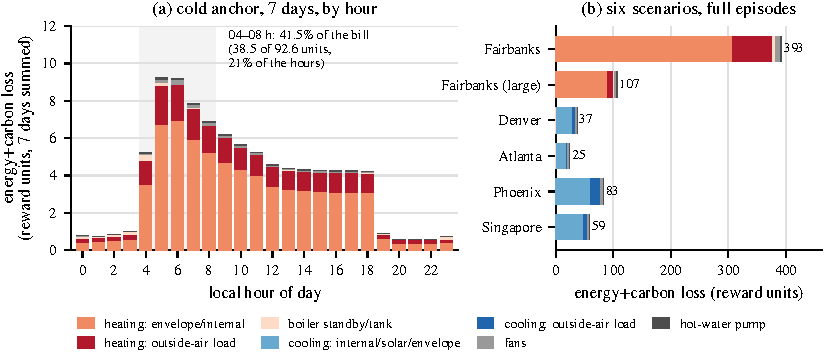
\includegraphics[width=0.92\linewidth]{figures/anatomy.pdf}
\captionof{figure}{Reward anatomy for a controller whose comfort term is already $0.6\,\%$ of its
loss. \textbf{(a)} The public anchor: energy-plus-carbon loss by local hour, stacked by
mechanism---envelope reheat (light) plus the outside-air share of the same reheat
(dark), $41.5\,\%$ of it in the pre-dawn 04--08\,h block, $21\,\%$ of the hours.
\textbf{(b)} The same decomposition for one full-length episode per climate; three
scenarios hold $83\,\%$ of the $702.9$-unit total (Appendix~\ref{app:energy}). Each bar
is a partition of the reward's own terms, reconciled below $1\e{9}$ relative.}
\label{fig:anatomy}
% src: paper/figures/anatomy.py reading results/ef_shipped/{*.json,*.npz} (shipped sim, CtrlW)
\end{center}

\paragraph{The warm stations: nothing to release.}
\label{app:cooling}
The release is inert on the warm stations because both conditions it exploits are
heating-only. On three seven-day warm anchors (CtrlW5-278, shipped) the chiller is
$93$--$95\,\%$ of the bill and the plant is already off when the building is empty
(Phoenix: $0.5\,\%$ of chiller energy at night, $0.0\,\%$ at weekends). The coil is billed at a
constant COP of 3.5 with no capacity limit, so there is no analogue of
Eq.~\eqref{eq:mult}: only airflow matters, and both airflow floors bind---the supply-air
setpoint sits at the 285\,K bound of the action space on $100$, $97.5$ and $91.8\,\%$ of live
AHU-steps (Phoenix, Singapore, Atlanta) and recirculation at the $0.70$ device cap on
$97$--$100\,\%$. Raising the unoccupied ceiling is bit-identical (it is never reached); riding
the band's top $0.12$\,K costs $5.0$ units on Phoenix, because the margin is the tracking error
and the reward prices an occupied kelvin at about 92 units a week against $0.62$ of cooling;
pre-cooling into cheap hours loses $3.9$--$6.9$, because the electricity term is
price-normalised (moving all of a week's cooling to its cheapest hour is worth $0.91$ of
$24.6$ units); a night flush is inert where nights are warm and loses where it fires; and
supply-air, reheat and static-pressure resets are outside the action space. Pre-cooling and
the night flush are the switches of CtrlW6, both off by default.
% src: docs/cool_gap.md; results/cool_*; policies/ctrl_w6.py (refutation knobs, inert defaults)

\section{Frost exposure}
\label{app:frost}

The measurements behind \S\ref{sec:frost}, on the six \cn{dev30} Fairbanks scenarios at
8\,641 steps, recorded by stepping the episode exactly as the evaluation runner does
and reading only the zone-average temperatures (no monkeypatching, no extra reward
call; the recorder reproduces the evaluation total to four decimals in every
configuration where both exist). \emph{h-any} is hours in which any room is below the
threshold, \emph{zone-h} room-hours.

\begin{center}
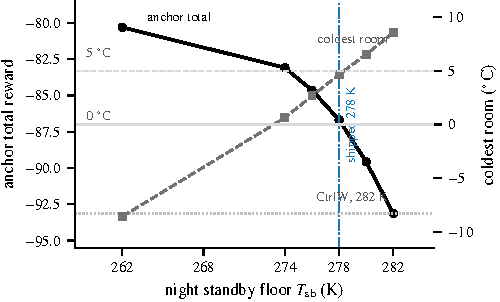
\includegraphics[width=0.62\linewidth]{figures/frost.pdf}
\captionof{figure}{Price of a frost floor on the anchor (2\,016 steps): anchor total reward (left)
and the coldest room temperature the episode reaches (right) against the night standby floor,
CtrlW5's other knobs fixed. On the anchor no room freezes from 274\,K up; 278\,K also keeps the
three cold 30-day scenarios above $+4.5\,^\circ$C, and a $\ge5\,^\circ$C setpoint floor needs 280\,K.}
\label{fig:frost}
\end{center}
% src: docs/control_gap.md §8.2 (sweep), §8.1 (minimum temperatures)

\begin{center}
\centering
\captionof{table}{Frost exposure and its price on the three cold \cn{dev30} Fairbanks scenarios
(\cn{building\_train\_\{1,2,8\}/fairbanks\_\{1,2,8\}}, 8\,641 steps each); the other three never leave
the band, so the floor is inert there. \emph{h-any} is hours in which any room is below the
threshold, \emph{zone-h} room-hours, and \emph{mean} the mean of $|\tfrac1T\sum_t r_t|$ over the
three. Over all six Fairbanks scenarios the set scores are 0.015653 (CtrlW), 0.015063
(CtrlW5-278, $-3.8\,\%$) and 0.014733 (CtrlW5-262, $-5.9\,\%$).}
% src: scratch/ControlGap/frost_*.json (not released; steps=8641 except the fairbanks_1 CtrlW5-262 cell, from docs/control_gap.md §8.1)
\label{tab:frost}
\footnotesize
\setlength{\tabcolsep}{3.5pt}
\begin{tabular}{@{}lcccccc@{}}
\toprule
Controller & coldest room & h-any $<5\,^\circ$C & h-any $<0\,^\circ$C & zone-h $<0\,^\circ$C & mean & $\Delta$ vs CtrlW \\
\midrule
CtrlW (282\,K)        & $+8.53$  & 0.0   & 0.0   & 0      & 0.027436 & --- \\
CtrlW5-278 & $+4.56$  & 459.8 & 0.0   & 0      & 0.026384 & $-3.8\,\%$ \\
CtrlW5-262 (no frost floor) & $-11.21$ & 496.1 & 274.9 & 2681.8 & 0.025724 & $-6.2\,\%$ \\
\bottomrule
\end{tabular}
\end{center}

\section{Reproducibility}
\label{app:repro}

Result directories contain one JSON per scenario with the score components, the
hour-of-day and weekday/weekend decomposition and the metering-hook output; every
entry we measured in Tables~\ref{tab:main}--\ref{tab:frost} is read from them, and
Figures~\ref{fig:mult}--\ref{fig:frost} are drawn from stored rollouts by
\texttt{paper/figures/\{multiplier,frost,anatomy\}.py}, with no simulator calls. The base controller is ported from
the public notebook \citep{wu2026alpha075} under Apache-2.0; with our flags off it
reproduces our run of its author's notebook on dev30 to the last digit (0.0075040), which is the parity
check we ran before adding anything.

\paragraph{Provenance.} The shipped tree is the starter kit at commit \texttt{95cea5b}
(2026-10-19, including the tracker fix of PR~\#1); the corrected tree adds PR~\#2 and PR~\#3
\citep{stncsn2026pr2,stncsn2026pr3}, frozen as patches and applied by \texttt{sbx/make\_sims.sh}.
Generated buildings are the first 24 kit-generator seeds from 5000 that fall inside the shipped
zone and air-handler ranges (5001--5025 for \cn{gen\_train}, 5026--5046 for \cn{gen\_hold}),
materials seed 20261105 (\texttt{sbx/make\_pool.py}); the external strips are described in
Appendix~\ref{app:weather}. Occupancy runs on the kit's seed 17321, and the reseeds use 12345 and
777; episodes are 8{,}640 scored steps plus a terminal one (result files report 8{,}641). The anchor CMA-ES (\texttt{cma} 4.5.0) searched CtrlW4's 16 knobs scaled to $[0,1]$ at
$\sigma_0=0.05$, population 12, seed 7, for 150 evaluations, starting from the best of 40 random
points, with the default point injected in every population. The kit's other reference
controllers are weaker than \cn{pid\_water} by its own shipped returns (fixed setpoint 0.0659,
PI 0.0674, bang-bang 0.2252), a file that puts \cn{pid\_water} at 0.05414 against our re-run's
0.05498 (25 scenarios at 0.054363 and 5 re-runs at 0.058058), so read them as indicative. CtrlX is \texttt{policies/ctrl\_x.py}, whose docstring
and parameter comments state each mechanism with its evidence; every run of its development,
kept or not, is logged in \texttt{docs/ctrlx\_experiments.md}, and the result directories behind
its numbers are under \texttt{results/ctrlx/}.

\paragraph{Commands.} With \texttt{PY=starter-kit/.venv/bin/python} in the root of the repository
(\url{https://github.com/MorS1337/sb26-stop-heating}; its README gives the setup):
{\footnotesize
\begin{verbatim}
$PY -m sbx.evalrun --policy policies.ctrl_w5:CtrlW5 --params '{"standby_minimum": 278.0}' \
    --set dev30 --steps 8641 --sim shipped --tag ctw5frost_dev30_shipped
$PY -m sbx.evalrun ... --sim corrected            # the corrected tree
$PY -m sbx.evalrun ... --set gen_hold ext_hold    # the 49 holdouts
$PY -m sbx.evalrun ... --cenv fused --fast        # the exact C step, same totals
$PY -m cenv.verify.gate trace --scenario building_train_8/fairbanks_8 --cenv fused --out t8_c
$PY -m kaggle.remote.remote_eval --policy ... --set dev30 --shards 4 --cenv fused --fast
$PY kaggle/build_notebook.py --policy policies/ctrl_w5.py:CtrlW5 \
    --param standby_minimum=278.0 --slug sbx-ctrl-w5f   # the CtrlW5-278 leaderboard entry
$PY -m sbx.arbench                                    # the CtrlX development benchmark
$PY -m sbx.evalrun --policy policies.ctrl_x:CtrlX --set dev30 --steps 8641 --sim corrected \
    --cenv fused --fast --tag ctrlx_dev30_corrected   # CtrlX; add --params for an ablation
$PY kaggle/build_notebook.py --policy policies/ctrl_x.py:CtrlX --slug sbx-ctrl-x   # 58217472
$PY kaggle/build_notebook.py --policy policies/ctrl_x.py:CtrlX --slug sbx-ctrl-x-hold \
    --param water_idle_hold=true --param water_peak_hold_hours=30.0 \
    --param water_rise_guard_K=2.5 --param water_offpeak_floor=0.0      # tank hold, 58217787
\end{verbatim}}

\paragraph{Machines and numerics.} Local runs used an Apple M3 and a Ryzen~5 5600X (WSL2); the
30-scenario and holdout sweeps also ran on Kaggle CPU kernels, at most four at a time. The fused
step is compiled with \texttt{-O3 -ffp-contract=off -fno-fast-math}---no FMA contraction, no
reassociation---the flags under which it is bit-identical to the Python step on each machine.
Across machines (arm64 with Accelerate against x86-64 with OpenBLAS) the same episode differs by
up to $3.3\e{5}$ relative over 30 days---round-off amplified by the closed loop, e.g.\
$-93.12290938$ against $-93.12336623$ for the seven-day anchor---far below the printed precision
of $S$ and the reseed spread, but enough to turn ``identical'' into ``better'' or ``worse''; every
better/identical/worse count therefore compares runs from one machine.
% src: results/{mac_smoke_anchor_cf,pc_smoke_anchor_cf}; ctw4_dev30_shipped (Kaggle) vs ctrw_all (Mac): 11 scenarios within 3.3e-5
% Table abl rows CtrlW2/CtrlW4 re-paired on Kaggle against results/q8/ctrw_dev30_shipped_kg (2026-11-07)

\section{External weather}
\label{app:weather}

\cn{ext} replays hourly observations from Meteostat \citep{meteostat2024} for calendar
year 2023 at seventeen stations absent from the benchmark---Anchorage, Auckland,
Bangkok, Beijing, Chicago, Dubai, Helsinki, Houston, Las Vegas, London, Miami, Montreal,
Moscow, Reykjavik, San Francisco, Seattle and Tokyo---mapped to the benchmark's
weather-file schema with no other scenario field modified. Meteostat data are
distributed under CC~BY~4.0; derived weather files are redistributed under the same
terms with attribution to Meteostat and its data providers.

\end{document}
